\chapter{Cara Menggunakan Buku}

Dalam buku ini, terdapat beberapa istilah-istilah yang digunakan agar pembaca dapat lebih memahami isi buku ini lebih baik. Selain itu, hal ini juga dapat membuat pembaca memiliki fokus yang lebih terarah ketika mempelajari buku ini.

\begin{description}
	\item[Eksplorasi] Dalam kotak eksplorasi, pembaca diharapkan dapat mengeksplorasi mengenai permasalahan yang diberikan pada kotak tersebut. Jika pembaca tidak memahami mengenai cara menjawab permasalahan dalam kotak ini, pembaca dapat mencari referensi lain seperti buku matematika lainnya atau internet. Itulah tujuan dari kotak eksplorasi ini, agar pembaca dapat mencari referensi lain dan tidak terpatok pada buku ini saja.
	\begin{explbox}
		Coba cari tahu mengenai Generasi Steiner. Apa hubungannya dengan proses pensketsaan parabola?
	\end{explbox}
	\item[Peringatan] Dalam kotak peringatan, pembaca dapat melihat suatu informasi penting yang kadang dilewatkan. Terkadang dalam matematika, terdapat beberapa miskonsepsi. Oleh karena itu, kotak peringatan ini bertujuan agar pembaca tidak terjerumus ke dalam miskonsepsi tersebut.
	\begin{warningbox}
		Perhatikan bahwa $ \displaystyle{\int{\func{f}{x}\func{g}{x} \diff{x}}} \ne \displaystyle{\int{\func{f}{x} \diff{x}} \cdot \int{\func{g}{x} \diff{x}}} $.
	\end{warningbox}
	\item[Informasi] Dalam kotak informasi, pembaca dapat mengetahui hal-hal mengenai suatu materi. Biasanya berisi mengenai tips dan trik, cara cepat, atau asal-usul formula tertentu dalam materi tersebut.
	\begin{infobox}{Informasi}
		Penyebutan rumus kuadratik sebagai rumus abc di Indonesia terkadang dijadikan candaan bagi dosen/guru matematika.
		\begin{quote}
			"Jika Anda mencari 'abc formula' di internet, tidak akan ketemu itu. Orang luar tidak ada yang menyebutnya sebagai abc formula, tetapi quadratic formula." \\[4pt]
			- Prof. Hendra Gunawan, Dosen Matematika ITB
		\end{quote}
	\end{infobox}
	\item[Tokoh] Dalam kotak tokoh, pembaca dapat mengetahui tokoh-tokoh matematika yang berperan dalam pengembangan materi yang diajarkan dalam buku ini. Pembaca juga diharapkan dapat meneladani tokoh-tokoh tersebut dan bisa menjadikannya sumber inspirasi dalam karier matematika Anda.
	\begin{charbox}{Francois Viete}
		Viete adalah matematikawan Prancis yang mendalami aljabar. Viete dilahirkan di Fontenay-le-Comte, yang saat ini dikenal sebagai Vendee pada tahun 1540. Ia dikenal karena teorema Vieta yang dikembangkannya. Viete sendiri memiliki nama lain (nama latin) Fransiscus Vieta. Nama latin inilah yang merupakan dasar penamaan teorema Vieta tersebut.
		\tcblower
		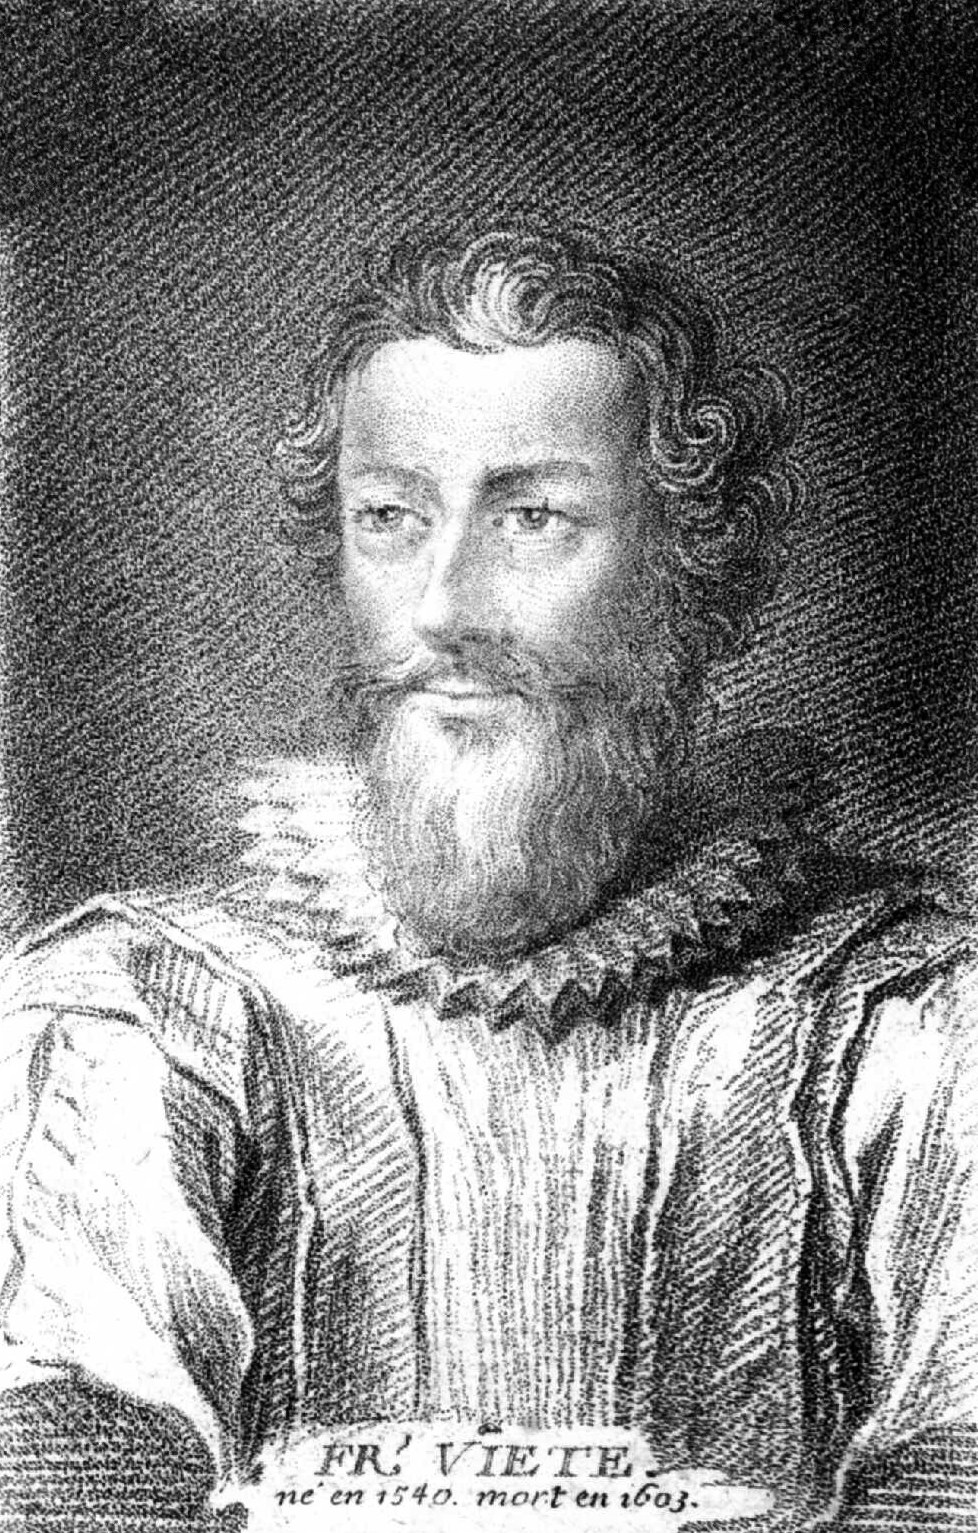
\includegraphics[width=\linewidth]{src/viete}
	\end{charbox}
	\item[Simbol Khusus Soal Latihan] Dalam soal-soal latihan, terdapat beberapa simbol khusus pada beberapa soal. Tujuan dari simbol khusus ini adalah agar pembaca dapat mengetahui jenis soal dan teknik penyelesaiannya. Beberapa simbol khusus tersebut adalah sebagai berikut.
	\begin{itemize}
		\item \probtype{$ \approx $}, yang berarti soal tersebut dapat diselesaikan dengan aproksimasi numerik.
		\item \probtype{C}, yang berarti penggunaan kalkulator (biasa) disarankan unuk menjawab soal tersebut.
		\item \probtype{CALC}, yang berarti soal tersebut kemungkinan besar harus diselesaikan dengan pengetahuan yang cukup mengenai kalkulus.
		\item \probtype{PF}, yang berarti soal tersebut selain harus diselesaikan, Anda juga harus membuktikan pekerjaan Anda.
		\item \probtype{EXPL}, yang berarti soal tersebut memerlukan eksplorasi lebih jauh mengenai materi yang telah dipelajari.
		\item \probtype{*}, \probtype{**}, dan \probtype{***} yang menunjukkan tingkat kesulitan soal tersebut.
	\end{itemize}
\end{description}